In diesem Kapitel soll der experimentelle Aufbau des gesamten Lasersystems und
dessen Kopplung an die Vakuumapperatur und den Quadrupol beschrieben werden.
Zunächst wird ein Überblick über das gesamte System gegeben (Abschn.
\ref{sec:gesamtaufbau}). Abschnitt \ref{sec:lasersystem} beschriebt den gesamten
optischen Aufbau inklusive Laserstabilisierung. Die Weiterverarbeitung der
Laserinformation und die Stabilisierung sollen in Abschn.
\ref{sec:elektronik_laserkontrolle} genauer betrachtet werden. Da
hard- und softwareseitige Implementierung der Laserkontrolle eng miteinander verknüpft
sind, kommt es zu Überschneidungen mit Kap. \ref{kap:software}, in dem die
softwareseitige Realisierung genau erklärt wird. In Abschn.
\ref{sec:vakuumapparatur_qms} und \ref{sec:messdatenverarbeitung} wird kurz
auf die verwendete Vakuumaparatur, dem daran gekoppelten
Quadrupolmassenseperator und die Messdatenverarbeitung eingegangen.
Abschnitt \ref{sec:vergleich_mit_altem_system} gibt einen kurzen Vergleich mit dem
bisher verwendeten, alten System.

\section{Gesamtaufbau}\label{sec:gesamtaufbau}
\begin{figure}[h]
 	\centering
 	\fbox{\parbox{\dimexpr \linewidth - 2\fboxrule - 2\fboxsep}{
 	\centering
	    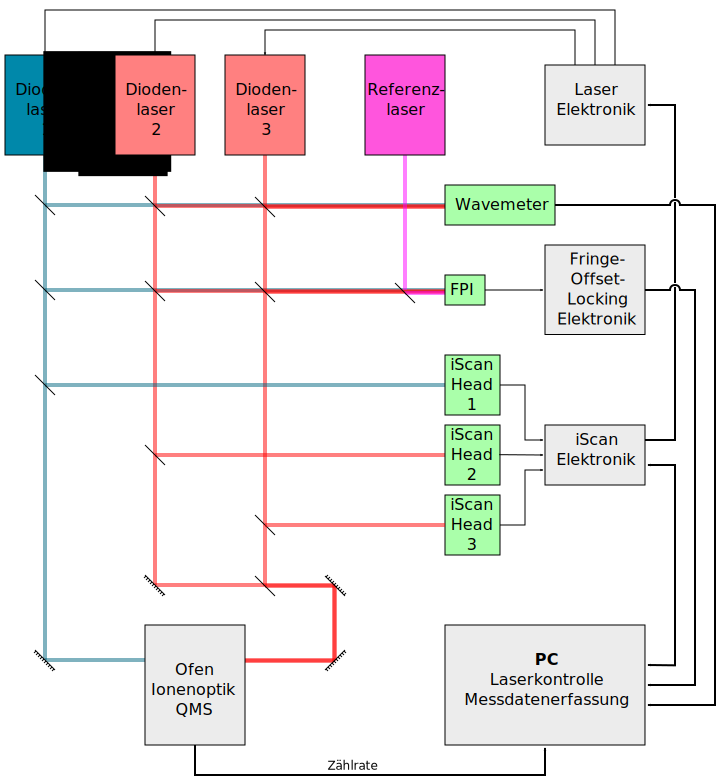
\includegraphics[width=\textwidth-2cm]{gfx/experimenteller_aufbau_gesamt}
	}}
	\caption[Gesamter experimenteller Aufbau, schematisch]{Gesamter experimenteller
	Aufbau des Systems (schematisch).}\label{fig:experimenteller_aufbau_gesamt}
\end{figure}
Abbildung \ref{fig:experimenteller_aufbau_gesamt} zeigt schematisch den gesamten
Aufbau des Systems. Das zur resonanten Anregung nötige Licht wird mit drei
Diodenlaser erzeugt. Der größte Teil des Lichts wird möglichst
direkt in die Vakuumaparatur geführt, die aus einem Ofen für das Ausheizen der
Atome, einer Ionenoptik für die Kontrolle der erzeugten Ionen und einem
Quadrupolmassenseperator (QMS) zur Massenselktion der Ionen besteht.
Die Einstrahlung der Laser erfolgt aus den in Abschn. \ref{sec:linienprofil}
erleuterten Gründen transversal zum aus dem Ofen austretenden kollimierten Atomstrahl.
Abgriffe der Hauptstrahlen führen das Laserlicht eines jeden Lasers in ein
Wavemeter, das die Absolutwellenlängen liefert und an einen PC weiterleitet.
Zwei jeweils weitere Abgriffe führen die Strahlen in die Optiken iScan Heads und FPI der zwei verwendeten
Laserstabilisierungen. Die dort erzeugten Signale werden an die jeweilige Elektronik
weitergeleitet. Die Elektronik eines iScan Heads ist die iScans control units, die direkt an die Elektronik des entsprechenden Laser
angeschlossen ist und sowohl die Spannung des Laserpiezos als auch den Strom
der Laserdiode moduliert. Die Elektronik des Fringe-Offset-Locking bereitet die
analogen Signale des FPIs digital auf und leitet sie weiter an den PC, der
gleichzeitig mit den iScan control units bidirektional verbunden ist und die
Regelung der iScan-Sollwerte übernimmt. Weiterhin kann mit dem PC die Zählrate
der Ionen, die einzeln durch ein hinter dem QMS angebrachtes Channeltron
detektiert werden, aufgenommen werden. Die Steuerung des Massenseperators
bezüglich der Einstellung bzw. des Scans bestimmter Massen durch den PC wurde im
Rahmen dieser Arbeit noch nicht realisiert, soll aber nachträglich implementiert
werden. Alternativ wird hierfür bis zum Abschluss dieser Arbeit noch ein PC des
Vorgängersystems verwendet.

\section{Lasersystem}\label{sec:lasersystem}
\begin{figure}[h]
 	\centering
 	\fbox{\parbox{\dimexpr \linewidth - 2\fboxrule - 2\fboxsep}{
 	\centering
	    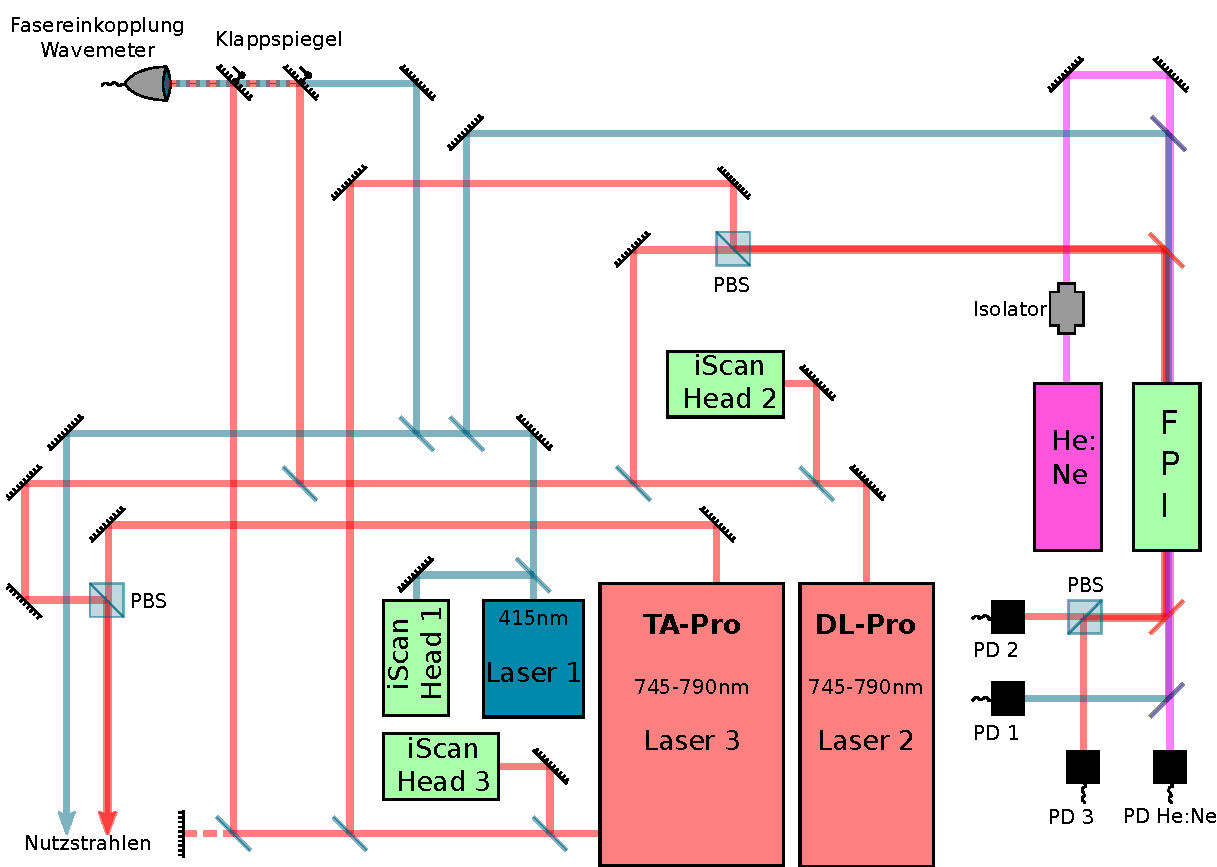
\includegraphics[width=\textwidth-2cm]{gfx/experimenteller_aufbau_lasersystem}
	    }}
	\caption[Experimenteller Aufbau des Lasersystems, schematisch]{Experimenteller
	Aufbau des Lasersystems
	(schematisch).}\label{fig:experimenteller_aufbau_lasersystem}
\end{figure}
\begin{figure}[h]
 	\centering
 	\fbox{\parbox{\dimexpr \linewidth - 2\fboxrule - 2\fboxsep}{
 	\centering
	    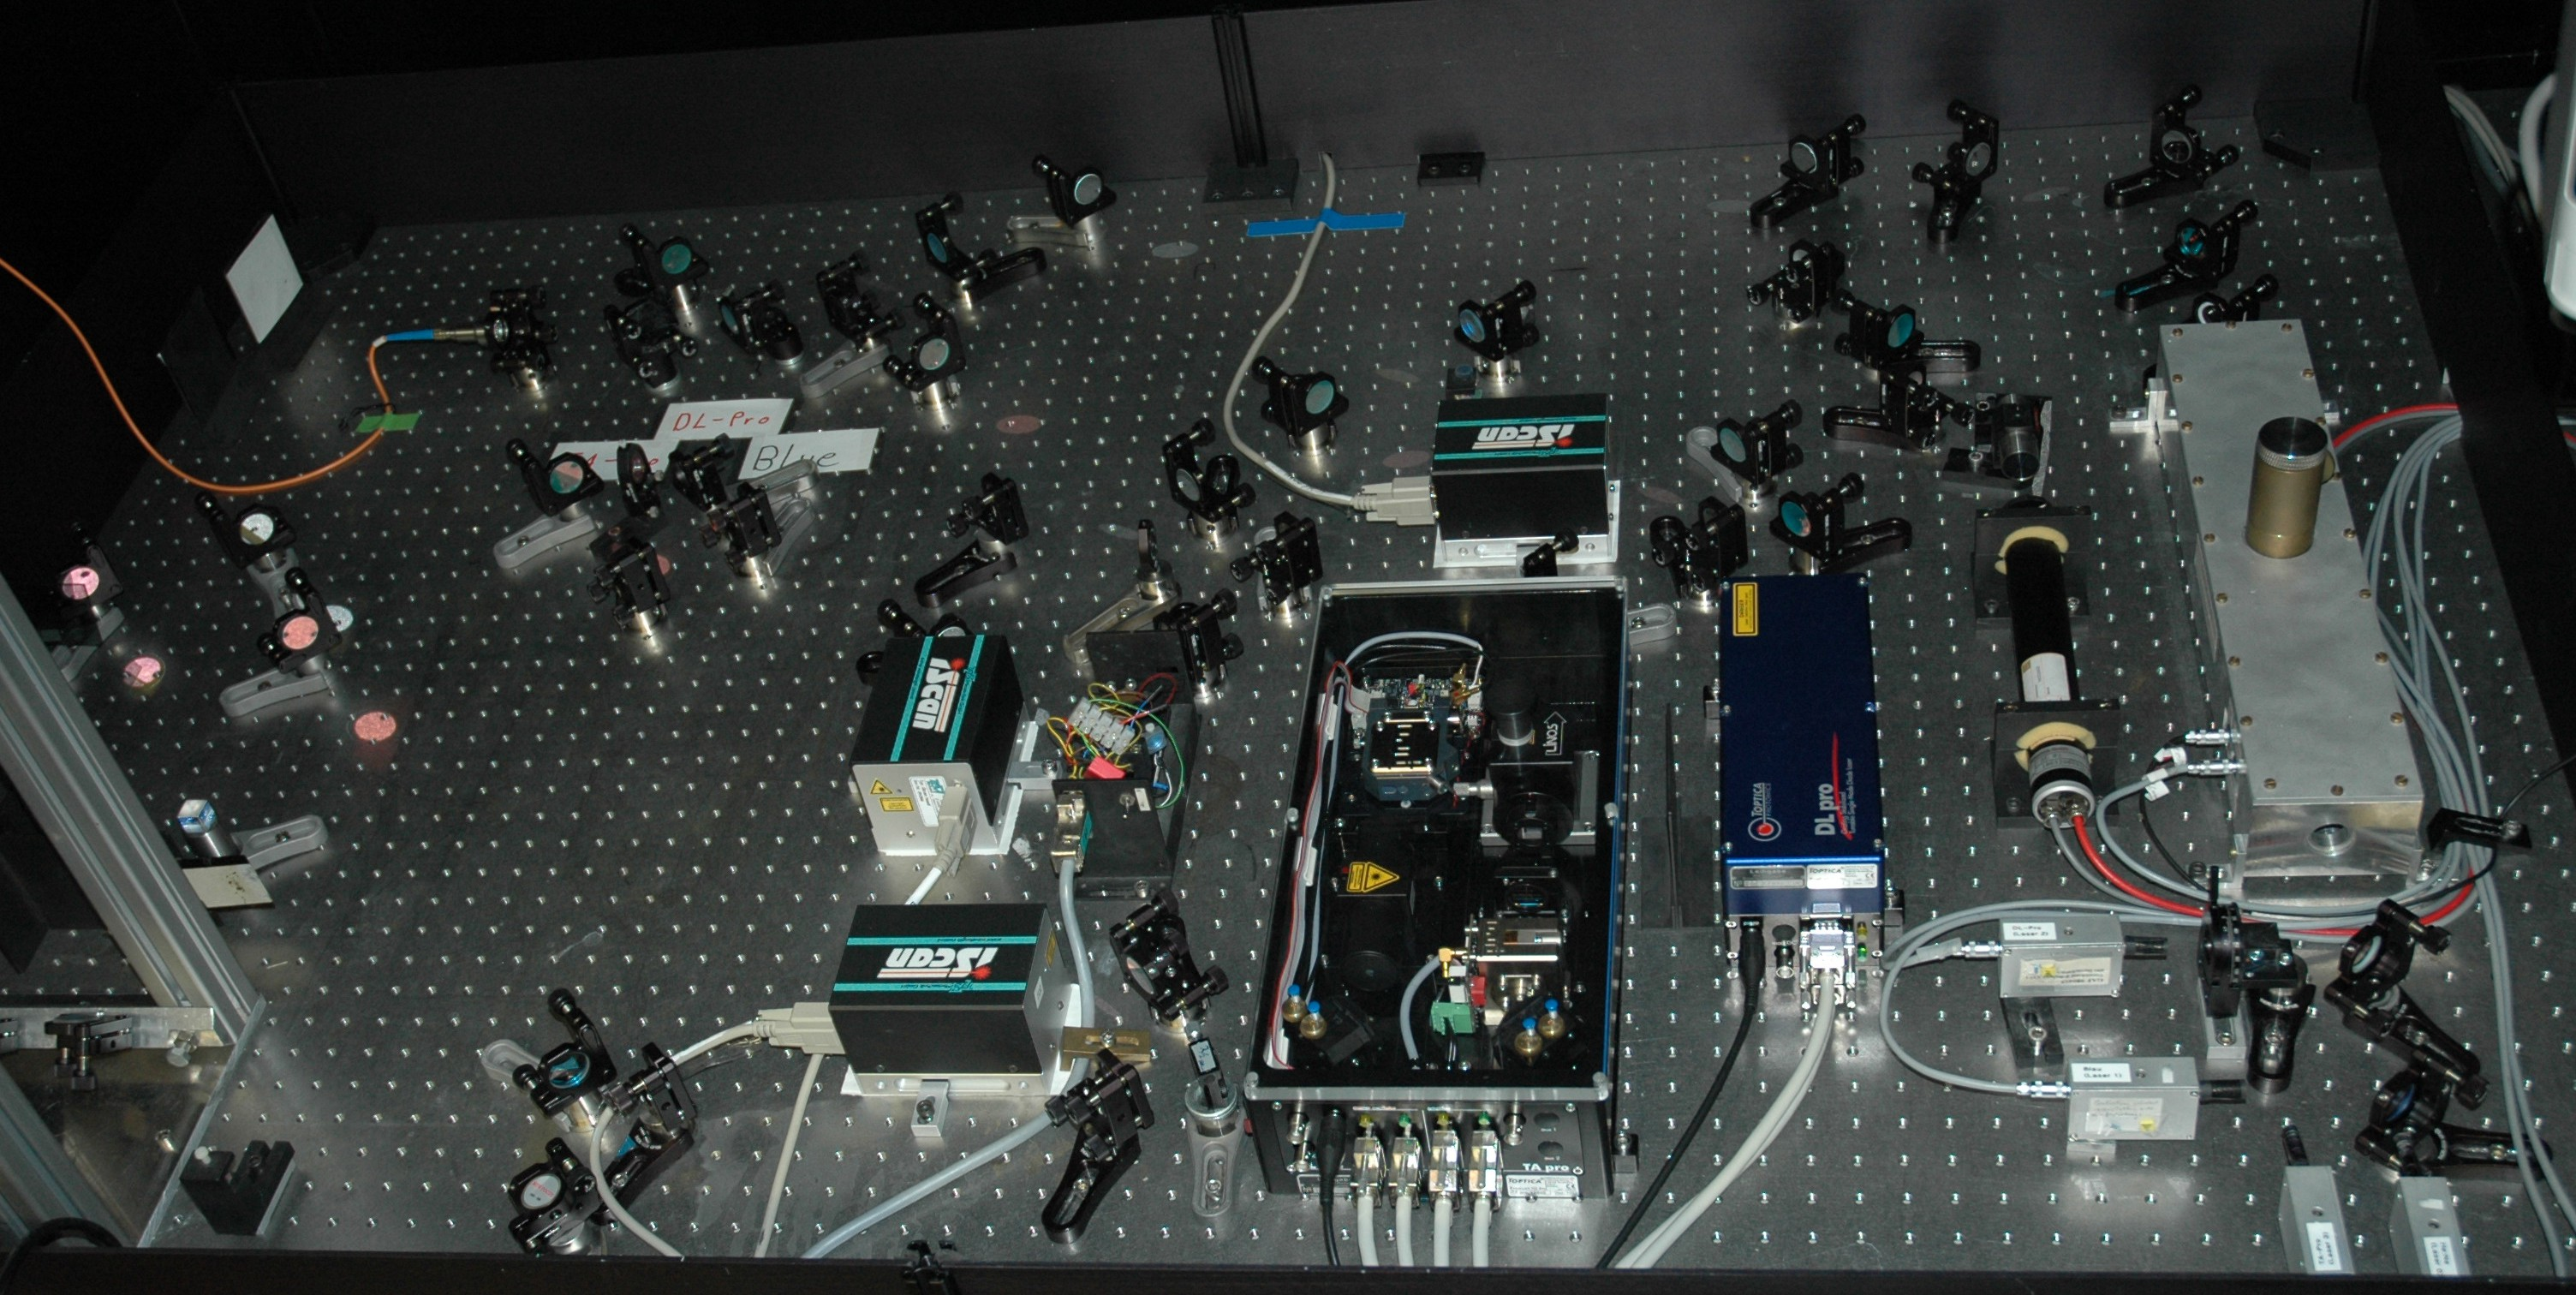
\includegraphics[width=\textwidth-0.5cm]{gfx/experimenteller_aufbau_lasersystem_foto}
	    }}
	\caption[Experimenteller Aufbau des Lasersystems -
	Foto]{Foto des
	verwendeten Lasersystems.
	Eingezeichnet sind die
	Strahlengänge der Laser.}\label{fig:experimenteller_aufbau_lasersystem_foto}
\end{figure}
%TODO: !lambda-halbe-plättchen etc.
Ein detaillierter Aufbau des Lasersystems wird schematisch durch Abb.
\ref{fig:experimenteller_aufbau_lasersystem} veranschaulicht und ist als
Fotografie in Abb. \ref{fig:experimenteller_aufbau_lasersystem_foto} noch einmal
zu sehen.\par
\begin{figure}[h]
 	\centering
 	\fbox{\parbox{\dimexpr \linewidth - 2\fboxrule - 2\fboxsep}{
 	\centering
	    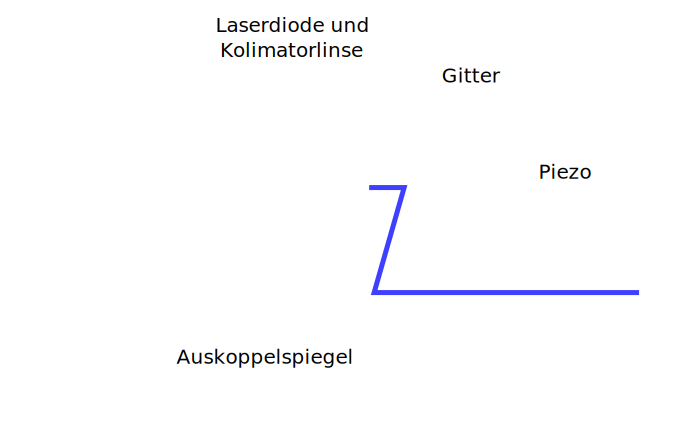
\includegraphics[width=\textwidth-1cm]{gfx/experimenteller_aufbau_diodenlaser_foto}
	    }}
	\caption[Diodenlaser - Foto]{Diodenlaser mit
	$405\,$nm-Diode und externen
	Resonator (Laser für den ersten
	Anregungsschritt).
	Eingezeichnet sind
	Laserdiode mit Kolimator,
	Gitter, Piezo,
	Auskoppelspiegel und
	Strahlengangd des
	Laserlichts.}\label{fig:experimenteller_aufbau_diodenlaser_foto}
\end{figure}
Das Laserlicht für den ersten Anregungsschritt wird in einem nach dem
Littrow-Design gebauten Diodenlaser erzeugt. Eingebaut ist eine blaue
$405\,$nm-Laserdiode mit einem Verstärkungsprofil von $\pm1\,$nm bei
zugeschalteten externen Resonator (siehe Abb.
\ref{fig:experimenteller_aufbau_diodenlaser_foto}). Der modensprungfreie Verstimmungsbereich ist mit $15\,$GHz spezifiziert. In manchen Moden wurden allerdings auch Verstimmungsbereiche
von bis zu $20\,$GHz erreicht. Das Laserlicht des zweiten und dritten
Anregungsschritts wird mit zwei kommerziellen, ebenfalls im Littrow-Design
gebauten, roten Diodenlasern der Firma Toptica erzeugt.
Beide Dioden haben ein spezifiziertes Verstärkungsprofil von
$745\,$nm bis $790\,$nm und einen modensprungfreien Verstimmungsbereich von bis
zu $30\,$GHz, was bestätigt wurde. Weiterhin kann das Laserlicht der Diode für
den dritten Anregungsschritt mit einem Trapezverstärker wahlweise bis auf eine
Leistung von $1,5\,$W verstärkt werden. Neben dem leistungsstarken Nutzstrahl
gibt es noch die Möglichkeit, einen Teil des zum Injection-Seeding verwendeten
Masterlaserstrahl abzugreifen (links unten am TA-Pro in Abb.
\ref{fig:experimenteller_aufbau_lasersystem}). Für den ersten bzw.
zweiten Anregungsschritt können ca. $7\,$mW bzw. ca. $60\,$mW bei Diodenströmen von ca. $35\,$mA bzw. ca.
$120\,$mA erreicht werden, was für die Untersuchung von Uran-Isotopen
ausreichend ist. Die Sättigungsleistungen sind im ersten Schritt $<1\,$mW, im
zweiten Schritt wenige mW und im dritten Schritt wenige $100\,$mW. Tabelle \ref{tab:laser_spezifikationen} listet noch einmal alle
Laser-Spezifikationen auf.
%TODO: !!Referenz zu Lasermanuals / Diodenmanuals
\par
\begin{table}
	%Summe der Breiten muss 0.91 mal \textwidth sein.
	\begin{tabular}{p{0.23\textwidth}|p{0.24\textwidth}p{0.24\textwidth}p{0.24\textwidth}}
		\toprule
		& Laser 1 & Laser 2 & Laser 3\\
		\midrule[1px]
		\hline
		Bezeichnung & Eigenbau & DL-Pro & TA-Pro\\
		Wellenlänge & $405\pm1\,$nm & $745\,$-$790\,$nm & $745\,$-$790\,$nm\\
		max. Leistung & $7\,$mW & $60\,$mW & $1,5\,$W\\
		nötige Leistung & $<1\,$mW & $xx\,$mW & $xxx\,$mW\\
		Externer Resonator & Littrow & Littrow & Littrow\\
		\bottomrule[1px]
	\end{tabular}
	\caption[Spezifikationen der verwendeten Diodenlaser]{Spezifikationen der
	verwendeten Diodenlaser}
	\label{tab:laser_spezifikationen}
\end{table}
Die Teilstrahlen für die Stabilisierung der iScans werden auf Grund der in
\ref{subsec:iScan} erklärten Empfindlichkeit auf räumliche Drifts möglichst
direkt in die iScan Heads geführt, damit die Hebelwirkung bei Drifts möglichst
gering ist. Für das iScan für Laser 3 muss die Polarisation mit einem
$\nicefrac{\lambda}{2}$-Plättchen gedreht werden.\par Die Abgriffe für das
Wavemeter des Typs \textit{WS Ultimate} von der Firma \textit{High Finesse}
müssen mit Klappspiegeln einzeln ausgewählt werden, da immer nur das Licht eines Lasers im Wavemeter analysiert werden kann. Da das Wavemeter eine
Genauigkeit von $40\,$MHz hat
\cite{wavemeter_hardware_guide}, würde es zur Frequenzstabilisierung nicht genügen, ist aber für das Finden von Resonanzen und wie schon erwähnt zum Berechnen der Relativfrequenzen nach Gl. \eqref{eq:FPI_frequenzdrift_03}
ausreichend.\par
Für das Fringe-Offset-Locking muss das Licht aller drei zu stabilisierenden
Laser vor dem FPI zusammengeführt und danach wieder getrennt werden. Da die
Wellenlängen von Laser 2 und 3 sehr nahe beieinander liegen, muss das Licht
dieser Laser mit Polarisationsstrahlteiler zusammengeführt und getrennt werden.
Dabei ist zu beachten, dass die Verluste durch die jeweils falsche Polarisation
der Laser möglichst gering ist, was durch optionales Drehen der
Polarisation mit $\nicefrac{\lambda}{2}$-Plättchen möglich ist. Die Überlagerung
mit dem blauen Licht des ersten Lasers und dem des He:Ne-Lasers kann mit
dichroitischen Spiegeln realisiert werden. Diese sind dafür ausgelegt, Licht
bestimmter Wellenlängenbereiche zu reflektieren, während Licht anderer  Bereiche
transmittiert wird. Die Trennung der Strahlen erfolgt nach demselben Prinzip.
Hinter dem gerampten FPI wird das Fringepattern aller vier Laser getrennt mit Photodioden aufgenommen. Das FPI hat nach Angaben aus dem Jahre 199x einen
freien Spektralbereich von $298,xx\,$MHz. Im nah-infraroten Bereich hat es die
größte Finesse, wohingegen im blauen Bereich die Finesse sehr schlecht ist.
Das Fringe-Offset-Locking ist damit zwar noch möglich, es wird allerdings
angestrebt, ein anderes Interferomter zu verwenden. Dieses wird momentan
noch in dem parallel laufenden alten System verwendet, das während dem
Entstehen dieser Arbeit noch als Referenzsystem eingesetzt und in
\ref{sec:vergleich_mit_altem_system} kurz beschrieben wird.\par
Die Hauptstrahlen werden an ein Pereskop geführt, über das das Licht in einen
anderen Raum an die Vakuum-Aparatur transportiert wird, wobei das Licht von
Laser 2 und 3 wieder durch Polarisationstrennung überlagert wird. Der
Strahltransport über das Pereskop ist Teil einer Vorablösung, da auf dem
Lasertisch der Vakuum-Aparatur noch das alte Lasersystem aufgebaut ist.\par
Der He:Ne-Laser ist gegen Rückreflexe aus dem FPI durch einen optischen Isolator
geschützt. Ebenso hat der dritte Laser vor dem Masterlaserabgriff und nach dem
Trapezverstärker je einen Isolator. Laser 1 und 2 haben momentan noch keinen
Isolator. Es soll jedoch in Zukunft jeweil ein Isolator zwischengeschaltet
werden.

\section{Elektronik der Laserkontrolle}\label{sec:elektronik_laserkontrolle} In
diesem Abschnitt wird die Verarbeitung der Signale zur Laserkontrolle schematisch erklärt. Für
Schaltpläne und interne elektronische Abläufe verschiedener Komponenten sei auf
den Anhang verwiesen. Abbildung \ref{fig:experimenteller_aufbau_elektronik_laserkontrolle} zeigt den
schematischen Aufbau der Elektronik für die Laserkontrolle.\par
\begin{figure}[h]
 	\centering
 	\fbox{\parbox{\dimexpr \linewidth - 2\fboxrule - 2\fboxsep}{
 	\centering
	    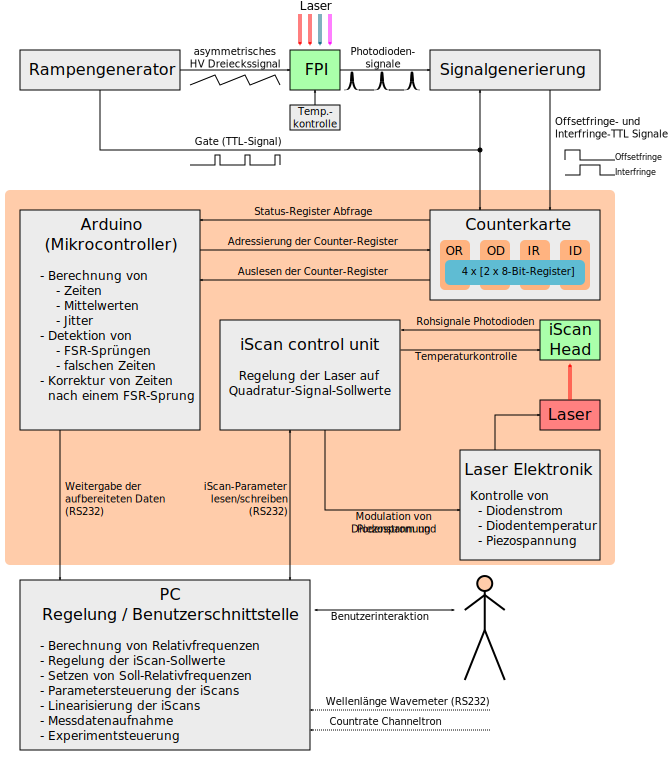
\includegraphics[width=\textwidth-2cm]{gfx/experimenteller_aufbau_elektronik_laserkontrolle}
	    }}
	\caption[Experimenteller Aufbau der Laserkontollelektronik,
	schematisch]{Experimenteller Aufbau der Elektronik der Laserkontrolle
	(schematisch).}\label{fig:experimenteller_aufbau_elektronik_laserkontrolle}
\end{figure}

\subsection{Signalgenerierung}\label{subsec:signalgenerierung}
Das FPI wird durch einen Rampengenerator in seiner Länge linear durchgefahren.
Dazu wird ein asymetrisches Dreieckssignal mit ca. $60\,$Hz erzeugt, welches das
wie in Abb.
\ref{fig:FPI_signal-zeitverlauf}(b) gezeigte Fringepattern für jeden Laser
an den Photodioden hinter dem FPI erzeugt. Außerdem gibt der Rampengenerator
ein TTL-Signal aus, des bei fallender Spannungsflanke HIGH und bei
steigender Spannungsflanke LOW ist. Die fallende bzw. steigende Flanke dieses
\textit{Gates} signalisiert also den Start bzw. das Ende der Spannungsrampe
und wird als Triggersignal verwendet. Die Photodiodensignale und das
Gate werden an einen Signalgenerator weitergegeben, welcher über Ableiten der
Fringesignale die wie in \ref{fig:FPI_signal-zeitverlauf}(d,e) gezeigten TTL-Pulse erzeugt.
Wie dies genau geschieht wird in Anh.
\ref{anh:kap:signalgenerierung_elektronik} beschrieben. Es ist weiterhin
möglich, eine \textit{Delay} in der Detektion des ersten Fringes einzustellen,
damit Nichtlinearitäten zu Beginn der Rampe umgangen werden.\par
Der im Folgenden beschriebene Ablauf ist für jeden zu stabilisierenden Laser
gleich (orange hinterlegter Bereich in Abb.
\ref{fig:experimenteller_aufbau_elektronik_laserkontrolle}). Daher wird dieser
Teil exemplarisch für einen Laser und den Referenzlaser beschrieben.

\subsection{Counterkarte}\label{subsec:counterkarte}
Die durch den Offsetfringe und Interfringe erzeugten
TTL-Pulse des sowohl zu stabilisierenden Lasers als auch des Referenzlasers
sowie das Gate werden an eine Counterkarte weitergeleitet. Diese besteht aus
vier 16-Bit-Countern und einem Taktgeber mit einstellbarer Taktrate ($1,25\,$,
$2,5\,$, $5\,$ und $10\,$MHz), wodurch unterschiedliche Zeitauflösungen möglich
sind ($0,8\,$, $0,4\,$, $0,2\,$ und $0,1\,$\textmu s).
Wird das Gate auf LOW gesetzt (Beginn der steigenden Spannungsflanke), werden
alle Counter freigeschaltet. Wenn die durch
das Delay etwas verzögerten TTL-Signale der Offsetfringes auf HIGH gesetzt werden, beginnen die
entsprechenden Counter der Offsetfringes (OR und OD) zu zählen. Beim Eintreten
der Offsetfringes werden die Counter gestopt und die Counter für die
Interfringezeiten gestartet (IR und ID). Auch diese werden beim Eintreten der
Interfringes gestopt. Am Ende der steigenden Spannungsflanke wird das Gate auf
HIGH gesetzt und die Counter werden gesperrt. Beim Stoppen eines jeden Counters
liegen die Counterwerte in jeweils 2x8-Bit-Registern (\textit{Upper Byte} und \textit{Lower Byte}) vor und es wird jeweils ein
\textit{Ready-Bit} gesetzt, welches Abrufbereitschaft der entsprechenden
Counterwerte signalisiert.\par
Die Ready-Bits sind über ein \textit{Statusregister} auslesbar. Die Adressierung
der einzelnen Counterregister wird über einen \textit{Adressbus} mit vier Bits
gesteuert, dessen Kodierung in Tab. \ref{tab:adressbus_kodierung} aufgeschlüsselt ist.
\begin{table}
	%Summe der Breiten muss 0.91 mal \textwidth sein.
	\begin{tabular}{p{0.1\textwidth}p{0.1\textwidth}p{0.1\textwidth}p{0.1\textwidth}|p{0.51\textwidth}}
		\toprule
		Enable & Addr. 1 & Addr. 2 & Addr. 3 & Wirkung\\
		\midrule[1px]
		\hline
		L & - & - & - & Adressierung deaktiviert\\
		H & L & L & L & Lower Byte Offsetfringe Referenzlaser\\
		H & L & L & H & Upper Byte Offsetfringe Referenzlaser\\
		H & L & H & L & Lower Byte Interfringe Referenzlaser\\
		H & L & H & H & Upper Byte Interfringe Referenzlaser\\
		H & H & L & L & Lower Byte Offsetfringe Diodenlaser\\
		H & H & L & H & Upper Byte Offsetfringe Diodenlaser\\
		H & H & H & L & Lower Byte Interfringe Diodenlaser\\
		H & H & H & H & Upper Byte Interfringe Diodenlaser\\
		\bottomrule[1px]
	\end{tabular}
	\caption[Adressierung Counterregister]{Aufschlüsselung der Adressierung der
	Counterregister}
	\label{tab:adressbus_kodierung}
\end{table}
Dabei sind \textit{Addr. 1}, \textit{Addr. 2} und \textit{Addr. 3} die
Adressleitungen. Über \textit{Enable} kann die Adressierung aktiviert und
deaktiviert werden. Sehr wichtig hierbei ist, dass bei einem Adressierungswechsel auf ein anderes
Counterregister die Adressierung immer deaktiviert werden muss. Andernfalls kann
es zur Zerstörung der Counter kommen. Schaltpläne und nähere Erleuterungen
zu der Counterkarte sind in Anh. \ref{anh:kap:counterkarte} zu finden.

\subsection{Datenaufbereitung (Arduino)}\label{subsec:arduino}
Die Auslese und Weiterverarbeitung der Werte muss nun bis spätestens zur
nächsten steigenden Spannungsrampe abgeschlossen sein, damit wieder die neuen
Rampensignale abgearbeitet werden können und es zu keinem Datenverlust kommt.
Dafür stehen der weiteren Datenverarbeitung im schlimmsten Fall nur $2\,$ms zur
Verfügung. Da bei einem PC mit klassischem Betriebssystem-Kernel wie Windows
NT$^\text{\textregistered}$ oder Linux die Prozessverwaltung auf Grund von unvorhersehbaren Interupts nie
deterministisch ist, ist es sehr unsicher, die Daten direkt mit einem PC zu
verarbeiten. Daher werden die Daten zunächst von einem Mikrocontroller
aufbereitet bevor sie weiter an einen PC gesendet werden. Ein Mikrocontroller
benötigt für gleiche Rechenvorgänge immer die gleiche Zeit, da es nie zu
unvorhergesehenen Interupts kommen kann. Als Mikrocontroller eignet sich dafür
hervorragend die Entwicklungsplattform \textit{Arduino$^\text{\textregistered}$}\footnote{http://www.arduino.cc}. Diese
wird verwendet, da sich das Projekt seitens der Elektronik und Software
auch nach Abschluss dieser Arbeit noch in der Entwicklungsphase befindet und der Arduino eine unkomplizierte Handhabung
und Programmierung bietet, was für Entwicklungszwecke gegenüber einem einfachen
Mikrocontroller-Chip vorteilhaft ist. Der hier eingesetzte
\textit{Arduino Mega 2560} mit dem Mikrocontroller-Chip \textit{ATmega2560}
bietet 54 digitale Ein- und Ausgänge. Er hat eine Taktrate von $16\,$MHz und
einen Flashspeicher von $256\,$kb für den binären Programmcode.
Die Programmierung erfolgt über eine frei verfügbare Entwicklungsumgebung.\par
Über das Statusregister erfährt der Arduino, ob einer der Counter das Zählen
beendet hat, adressiert dessen Register und liest diese über einen
8-Bit-Datenbus aus. Nach Ende einer steigenden Rampe, hat der Arduino im
schlimmsten Fall noch maximal $2\,$ms Zeit, um abschließende Berechnungen
auszuführen. Die Aufgabe des Arduinos ist es, die Zeiten $t_{OR}$, $t_{OD}$,
$t_{IR}$ und $t_{ID}$ zu berechnen und Mittelwerte über mehrer Rampenzyklen zu
bilden. Darüber hinaus wird der Laser-Jitter über mehrere Rampenzyklen
ermittelt, Sprünge in benachbarte FSRs des FPIs detektiert und Zeiten
korrigiert. Außerdem werden ungewöhnliche Zeiten verworfen. Wie dies genau
abläuft, soll in Kap. \ref{kap:software} erleutert werden. So geht möglichst
wenig Information über die Laser verloren, wobei gleichzeitig dem PC genügend
Zeit zur Verfügung steht, um die Regelung der iScan-Sollwerte abzuwickeln.

\subsection{PC - Regelung /
Benutzerschnittstelle}\label{subsec:pc_regelung_benutzerschnittstelle} Die
aufbereiteten Daten werden anschließend über eine RS232-Schnittstelle an einen mit Windows
7$^\text{\textregistered}$ aufgesetzten PC übermittelt, auf dem ein auf
\textit{Labview} basierendes Kontrollprogramm läuft. Labview übernimmt nun die endgültige Berechnung der
Ist-Relativfrequenzen und die Regelung auf die eingestellte Soll-Relativfrequenz
aller drei Laser über das Setzen der iScan-Sollwerte wie schon in Abschn.
\ref{sec:iscan_und_fringe-offset-locking} beschrieben wurde.
Dazu ist der PC wiederum über RS232-Schnittstellen an die iScan control units
angeschlossen. Es entsteht zwar wegen der Mittelung der Werte durch den Arduino
in wesentlich geringerer Rate Datenpakete für die Stabilisierung über den PC. Da
die Regelung über das Fringe-Offset-Locking aber ohnehin nur zum Ausgleichen der Fehler und Drifts
der iScans dient, ist diese etwas "`gemächlichere"' Regelung kein Nachteil.
Weiterhin übernimmt das Labview-Programm Monitoraufgaben der Laser,
Parametersteuerung der iScans, Messdatenaufnahme, Experimentsteuerung und
Linearisierung der iScans, was in Kap. \ref{kap:software} näher betrachtet wird.\par

\subsection{iScan control unit}\label{subsec:iscan_control_unit}
Neben der Regelung der Laser auf einen Sollwert bietet die iScan control unit
noch weitere Funktionen wie z.B. Frequenzscans und Datenaufnahme. Dieser
Abschnitt soll sich allerdings auf die Regelung der iScans beschränken. Weitere
Funktionen werden z.B. bei der Linearisierung der iScans benutzt (siehe Abschn.
\ref{sec:linearisierung_iscan}).\par
Abbildung \ref{fig:iscan_control_unit_regelelektronik} zeigt schematisch den
Teil der Elektronik der iScan control unit, der für die Regelung und die
Manipulation der Laserparameter zuständig ist. Die Peripherie-Elektronik und
detailierte Schaltungen wurden dabei bewusst ausgelassen, um die Übersicht zu
bewahren. Für Detailschaltungen sei auf das Hardwarehandbuch der iScans
verwiesen \cite{iscan_hardware_guide}.\par
\begin{figure}[h]
 	\centering
 	\fbox{\parbox{\dimexpr \linewidth - 2\fboxrule - 2\fboxsep}{
 	\centering
	    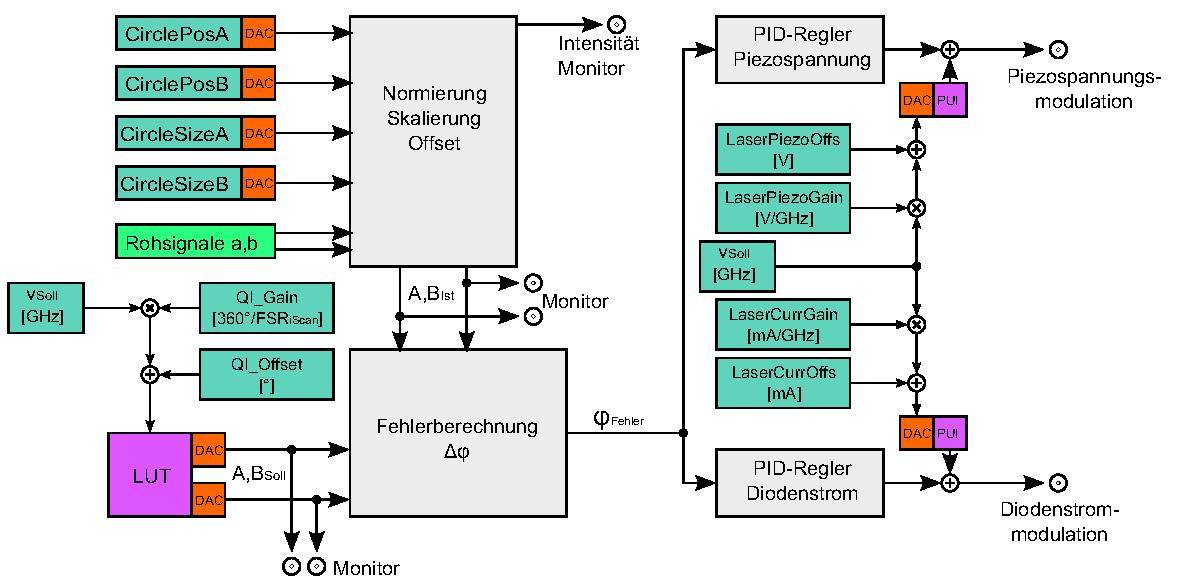
\includegraphics[width=\textwidth-0cm]{gfx/iscan_control_unit_regelelektronik}
	    }}
	\caption[Interner Aufbau der iScan control unit, schematisch]{Interner Aufbau
	der iScan control unit
	(schematisch).}\label{fig:iscan_control_unit_regelelektronik}
\end{figure}
Die türkisen Kästen in Abb. \ref{fig:iscan_control_unit_regelelektronik} stellen
digitale Parameter dar, die entweder zum Teil per Hand über eine Digitalanzeige
direkt an der iScan control unit oder über einen PC via RS232-Schnittstelle
ausgelesen bzw. programmiert werden können. Neben den hier angegebenen
Parametern gibt es eine Reihe weiterer Parameter, die im Hardwarehandbuch
nachgelesen oder mit dem Befehls-String \lstinline|VarDump| ausgelesen werden
können. Näheres zur softwareseitigen Kommunikation findet sich in Kap.
\ref{kap:software}. Über \textit{Digital-Analog-Converter} (DAC) können die
digitalen Werte in analoge Spannungen mit Einschränkunegn in Auflösung und
Maximalwerten übersetzt werden. Sowohl die digitalen Berechnungen als auch
die Übersetzungen zwischen analogen und digitalen Werten werden von einem
Mikrocontroller übernommen.\par
Ausgangspunkt der Regelschleife der iScans ist der digital angegebene Sollwert
der Relativfrequenz $\nu_{Soll}$, wobei die Null-Frequenz als Bezugspunkt eine
beliebige Laserfrequenz (siehe Wavemeter) sein kann. Der Sollwert kann auf
verscheidene Arten festgelegt werden. Die hier verwendete Variante ist das Festlegen des
Paramters \lstinline|ScanOffset|, welcher wie alle anderen Parameter mit der
Einheit Hertz eine Auflösung von $1\,$MHz hat. Weiterhin kann der Sollwert auch
ausgehend von \lstinline|ScanOffset| während einer Scanroutine des iScans
kontinuierlich geändert werden. Diese zweite Variante wird hier nur wie oben
erwähnt bei der Linearisierung der iScans eingesetzt. Um frequenzabhängige
Messungen zu betreiben, wird in dieser Arbeit lediglich ein
\lstinline|ScanOffset|-Wert gesetzt. Daraufhin werden die entsprechenden
Messdaten aufgenommen und anschließend der nächste \lstinline|ScanOffset|-Wert
gesetzt.\par
Der digital hinterlegte Wert für den FSR der iScans (Parameter
\lstinline|FSR|) wird verwendet, um eine lineare Abhängigkeit
\lstinline|QI_Gain| zwischen der Phase eines Quadraturkreispunktes und der
Frequenz herzustellen. Ein Offset wird durch den Parameter \lstinline|QI_Offset| erreicht. Es ergibt sich also ein Sollwert der Phase über
\begin{equation}\label{eq:iscan_soll_phase_berechnung}
	\phi_{Soll}=\nu_{Soll}\cdot\text{\lstinline|QI_Gain|}+\text{\lstinline|QI_Offset|}\,.
\end{equation}
Wie schon erklärt, wird dieser Wert nun über die LUT mit den die tatsächliche
Sollfrequenz repräsentierenden Werte $A_{Soll}$ und $B_{Soll}$ verknüpft. Über
DACs werden die analogen Werte an eine analoge Fehlerberechnungsroutine für die
Phase weitergeleitet.\par
Parallel dazu werden die Rohsignale des iScan Heads $a$ und $b$ normiert und
über die Skalierungs- und Offset-Parameter \lstinline|CircleSizeA|,
\lstinline|CircleSizeB|, \lstinline|CirclePosA| und \lstinline|CirclePosB| so
manipuliert, dass diese einen möglichst deckungsgleichen Quadraturkreis mit dem
Vorgabe-Quadraturkreis aus $A_{Soll}$ und $B_{Soll}$ bilden. Auch diese analogen
Spannungen $A_{Ist}$ und $B_{Ist}$ werden an die Fehlerberechnungsroutine
weitergegeben. Nebenbei können die Quadraturkreise bzw. Quadraturkreispunkte der
Ist-Spannungen $A_{Ist}$ und $B_{Ist}$ parallel zu denen der Soll-Spannungen
$A_{Soll}$ und $B_{Soll}$ durch den Monitor-Ausgang an einem Oszilloskop im
XY-Modus dargestellt werden wie in Abschn. \ref{subsec:iScan} beschrieben ist.
Ebenso kann die Laserleistung über den Intensitäts-Monitor-Ausgang überwacht
werden.\par Der analog berechnete Fehler für die Phase wird an die beiden
kontinuierlichen PID-Regler für Piezospannung und Diodenstrom übergeben. Die
Regelgrößen werden auf die schon in den gewollten Bereich verfahrenen
Piezospannungs- und Diodenstrommodulationsspannungen addiert. Ohne ein
Voreinstellen dieser Größen ist eine Regelung über größere Frequenzbereich nicht
möglich bzw. zu langsam. Die Voreinstellung erfolgt über die folgende
Parameterverknüpfung:
\begin{equation}\label{eq:iscan_PUs}
	\begin{split}
		U_{Piezo,mod}&=\nu_{Soll}\cdot\text{\lstinline|LaserPiezoGain|}+\text{\lstinline|LaserPiezoOffs|}\\
		I_{Diode,mod}&=\nu_{Soll}\cdot\text{\lstinline|LaserCurrGain|}+\text{\lstinline|LaserCurrOffs|}\,.
	\end{split}
\end{equation}
$U_{Piezo,mod}$ und $I_{Diode,mod}$ sind dabei die Änderungsgrößen der
Laserparameter. Die eigentlichen Modulationsspannungen
sind von diesen Größen verscheiden und müssen daher von dem sog.
\textit{Physical Unit Interface} (PUI) aus $U_{Piezo,mod}$ und $I_{Diode,mod}$ in Digitalwerte und weiter über DACs in die Modulationsspannungen übersetzt werden.
Selbstverständlich muss daher jedes PUI zunächst geeicht werden. Die
Vorgehensweise dazu wird in \cite{iscan_hardware_guide}
erklärt. Mit dem Setzen der Modulationsspannungen und dem folglichen Ändern der
Laserfrequenz ist die Regelschleife der iScans geschlossen.

\section{Vakuumapparatur /
Quadrupolmassenspektrometer}\label{sec:vakuumapparatur_qms}
In diesem Abschnitt soll kurz auf die verwendete Vakuumapparatur und das daran
gekoppelte Quadrupolmassenspektrometer (QMS) eingegangen werden. Ausführliche
Beschreibungen können der Arbeit \cite{blaum:1997:diplomarbeit} entnommen
werden. Abbildung \ref{fig:vakuumapparatur_foto} zeigt die Vakuumapparatur mit
einem Druck in der Größenordnung von $10^{-6}\,$mBar bis $10^{-8}\,$mBar.\par
\begin{figure}[h]
 	\centering
 	\fbox{\parbox{\dimexpr \linewidth - 2\fboxrule - 2\fboxsep}{
 	\centering
	    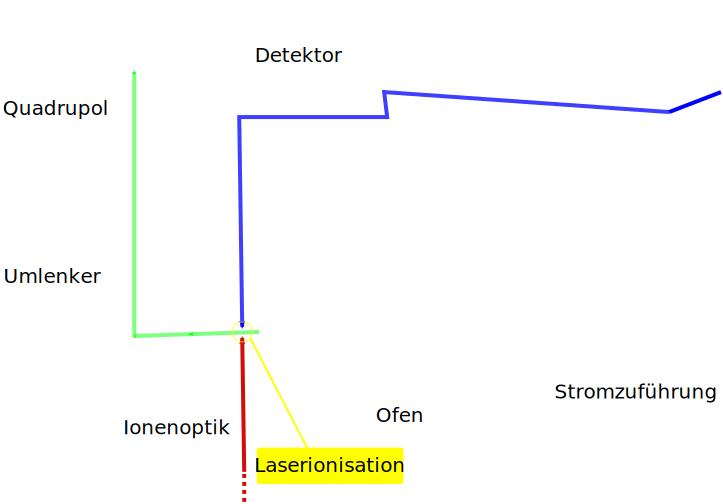
\includegraphics[width=\textwidth-0.3cm]{gfx/vakuumapparatur_foto}
	    }}
	\caption[Vakuumapparatur]{Vakuumapparatur: Eingezeichnet
	sind Atom- bzw. Ionenstrahl, Laserstrahlen,
	Ofen mit Stromzuführung, Wechselwirkungsregion, Ionenoptik, Umlenker,
	Quadrupol und Detektor.}\label{fig:vakuumapparatur_foto}
\end{figure}
Rechts befindet sich der Atomstrahlofen, der aus einem $50\,$mm langem
Graphitröhrchen mit einem (Innen-)Durchmesser von ($2,9\,$mm) $4,1\,$mm besteht \cite{raeder:2006:diplomarbeit}. Das Röhrchen lässt sich einseitig auf einen
Molybdänstab schrauben, der gleichzeitig als Stromzuführung dient. Die andere
Seite des Röhrchens ist Träger der zu untersuchenden Uran-Probe und wird leicht
gegen eine kleeblattförmige Blende gedrückt, die als Stromabführung dient. Alle
Stromführenden Elemente sind aus Kühlzwecken entweder wasserdurchflossene
Kupferblöcke oder werden von solchen umgeben. Der Ofen kann bei einem Strom von
bis zu $120\,$A bis auf $2300\,$K aufgeheizt werden. Der Ofen
ist momentan allerdings noch im Entwicklungsstatus, wobei sich die Konfiguration
in nächster Zeit teilweise ändern wird.\par
Der durch das Aufheizen der Probe nach links austretende Atomstrahl durchläuft
die Wechselwirkungszone mit den Lasern, in der durch Resonanzionisation
Laserionen erzeugt werden. Die Laser werden dabei transversal zum Atomstrahl
und wegend der Dopplerkompensation gegenläufig eingestrahlt. Die Ionen werden
mit Hilfe einer Ionenoptik abgesaugt und über einen Quadrupolumlenker im rechten Winkel in das QMS geführt und anschließend mit einem Kanalelektronenvervielfacher detektiert. Ionen, die ungewollt vor der
Wechselwirkungszone mit den Lasern enstanden sind (sog.
Oberflächenionen) werden mit Hilfe einer Repellerlinse, die auf positivem
Potential relativ zum Ofen liegt, abgeblockt.
So erreicht man bei ausgeschalteten Lasern eine Zählrate von Oberflächenionen in
der Größenordnung von $10^{-1}\,$ Ionen pro Sekunde.\par
Das QMS, auf das im folgenden Abschnitt \ref{subsec:quadrupolmassenspektrometer}
etwas näher eingegangen wird, filtert alle Teilchen außer die einer bestimmten
Masse aus. In der hochselektiven Resonanzionisationsspektroskopie ist dies auf
den ersten Blick nicht nötig, da nach der Wechselwirkungregion nur noch
Laserionen des Zielisotops weiter in das QMS geleitet werden, was auch
näherungsweise zutrifft. Um jedoch sicher zu sein, dass weder Ionen eines
falschen Isotops, noch Ionen des Restgases, des Ofenmaterials oder ionische
Moleküle anderer Massen detektiert werden, wird das QMS hinzugenommen.

\subsection{Quadrupolmassenspektrometer}\label{subsec:quadrupolmassenspektrometer}
%TODO: !QMS Bild
Ein QMS besteht aus vier mit radialem Abastand zum Zentrum $r$ angeordneten
äquidistanten runden Metallstäben wie in \ref{fig:quadrupolmassenspektrometer}
schematisch dargestellt ist. Zwei gegenüberliegende Stäbe liegen jeweils immer
auf demselben Potential
\begin{equation}\label{eq:qms_potential_0}
	\Phi_0(t)=\pm\left(U+V\cos{(\Omega t)}\right)\,,
\end{equation}
wobei das eine Stabpaar das obere und das andere Stabpaar das untere Vorzeichen
besitzt. Das Potential $\Phi_0(t)$ setzt sich aus einer konstanten Spannung $U$
und einer Wechselspannung $V\cos{(\Omega t)}$ mit der Frequenz $\Omega=1,2\,$MHz
zusammen. Zwischen den Stäben ergibt sich das ortsabhängiges Potential
\begin{equation}\label{eq:qms_potential_ort}
	\Phi_0(\vec{r},t)=\pm\left(U+V\cos{(\Omega
	t)}\right)\cdot\frac{x^2-y^2}{r^2}\,,
\end{equation}
das ortsunabhängig in z-Richtung ist. Aus der Bewegungsgleichung
\begin{equation}\label{eq:qms_bewegungsgleichung}
	m\ddot{\vec{r}}+e\vec{\nabla}\Phi(\vec{r},t)
\end{equation}
ergeben sich die \textit{Mathieu'schen Differentialgleichungen}
\begin{subequations}\label{eq:qms_mathieu}
	\begin{equation}\label{eq:qms_mathieu_01}
		\fracdd{x}{\xi}+(a_x+2q_x\cdot\cos{2\xi})\cdot x=0
	\end{equation}
	\begin{equation}\label{eq:qms_mathieu_02}
		\fracdd{y}{\xi}-(a_y+2q_y\cdot\cos{2\xi})\cdot y=0
	\end{equation}	
\end{subequations}
mit den Transformationsparametern
\begin{subequations}\label{eq:qms_mathieu_trsf}
	\begin{equation}\label{eq:qms_mathieu_trsf_01}
		\Omega t=2\xi
	\end{equation}
	\begin{equation}\label{eq:qms_mathieu_trsf_02}
		a_x=-a_y=\frac{8eU}{mr^2\Omega^2}
	\end{equation}
	\begin{equation}\label{eq:qms_mathieu_trsf_03}
		q_x=-q_y=\frac{4eV}{mr^2\Omega^2}\,.
	\end{equation}
\end{subequations}
Anstatt auf die exakten mathematischen Lösungen der Differenzialgleichungen
soll hier auf die direkte Folge daraus eingegangen werden. Die Lösungen der
DGLn können in zwei Klassen eingeteilt werden: stabile und instabile Lösungen.
Die Lösung für die Teilchen mit dem Ladungs-Masseverhältnis $\nicefrac{e}{m}$,
die den Quadrupol passieren, nennt man stabil. Alle anderen Lösungen sind instabil.
Trägt man nun die Parameter $a$ und $q$ gegeneinander auf, findet man in erster
Ordnung das Stabilitätsdiagramm aus Abb. \ref{subfig:stabilitaetsdiagramm_aq}.
\begin{figure}[h]
	\centering
	\fbox{\parbox{\dimexpr \linewidth - 2\fboxrule - 2\fboxsep}{
	\subfigure[]{
		\label{subfig:stabilitaetsdiagramm_aq}
		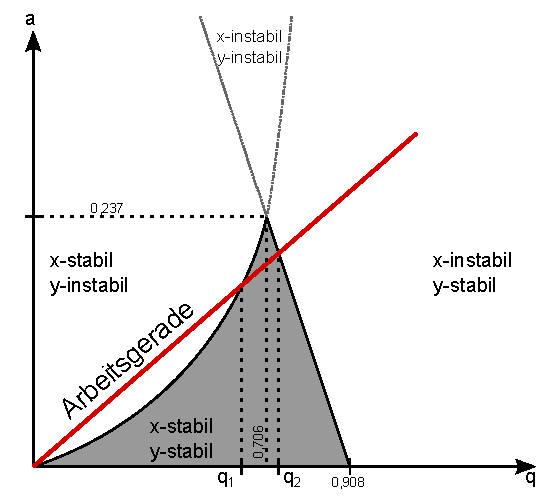
\includegraphics[width=(\textwidth-1cm)/2]{gfx/stabilitaetsdiagramm_aq}
  	}
	\subfigure[]{
		\label{subfig:stabilitaetsdiagramm_UV}
		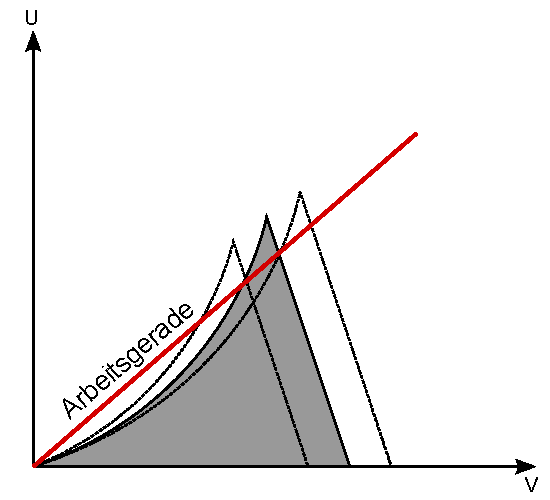
\includegraphics[width=(\textwidth-1cm)/2]{gfx/stabilitaetsdiagramm_UV}
  	}
	}}
	\caption[Stabilitätsdiagramm]{In (a) ist in grau das Stabilitätsdiagramm erster
	Ordnung in Abhängigkeit von den Parametern $a$ und $q$ eingezeichnet. Die
	gestrichelten Dreiecke in (b) sind die stabilen Bereiche von Teilchen mit
	anderen $\nicefrac{e}{m}$-Verhältnissen ($U$-$V$-Abhängigkeit).}
	\label{fig:stabilitaetsdiagramm}
\end{figure}
Nur die Teilchen, deren $a$ und $q$ im grauen
Bereich liegen, sind sowohl in x- als auch in y-Richtung stabil und werden nicht
ausgefiltert. Rechts davon sind diese Teilchen in x-Richtung instabil und in
y-Richtung stabil. Umgekehrtes gilt links von diesem Gebiet. Oberhalb des
Dreiecks sind die Lösungen in beide Dimensionen instabil. Der Quotient
$\nicefrac{a}{q}=\nicefrac{2U}{V}$ ist unabhängig von dem Ladungs-Masseverhältnis der Teilchen und kann somit als Steigung für die Arbeitsgerade in Abb.
\ref{fig:stabilitaetsdiagramm} dienen. Die Einstellung dieses Quotienten wirkt
sich auf das stabile Masseintervall $\Delta m=[m_1,m_2]$ aus, was
gleichbedeutend mit dem Intervall $[q_1,q_2]$ ist. Je schärfer die Arbeitsgerade die Spitze des
Stabilitätsdreiecks schneidet desto besser ist die Massenauflösung
$R=\nicefrac{m}{\Delta m}$. Die gestrichelten Stabilitätsdreiecke in
\ref{subfig:stabilitaetsdiagramm_UV} sind die der Teilchen mit anderen
$\nicefrac{e}{m}$-Verhältnissen, bzw. mit anderen Massen, wenn man davon
ausgeht, dass alle Ionen einfach positiv geladen sind ($U$-$V$-Abhängigkeit).
Mit einem simultanen Verfahren von $U$ und $V$ und Beibehalten des Verhältnisses
$\nicefrac{2U}{V}$ können die Spitzen der Stabilitätsdreiecke von Teilchen verschiedener Masse angefahren und die entsprechenden Teilchen
selektiert werden. Streng genommen liegen die Spitzen der
Stabilitätsdreiecke nicht auf einer Gerade, sondern einem Polynom höheren
Grades. Deshalb wäre es nötig, den Quadrupol für verschiedene Massebereiche
extra zu kalibrieren. Da zur Untersuchung der Uranisotope aber nur ein sehr
begrenztes Masseintervall nötig ist ($^{233}$U bis $^{238}$U), reicht eine
einmalige Kalibration für diesen Bereich.\par
Der hier verwendete QMS von der Firma \textit{ABB
Extrel} ist ausgelegt für einen Massebereich von $0\,$-$300\,$u. Die Massen
können durch ein Modulationsspanunngssignal (\textit{Masscommand}) über einen
DAC von einem PC aus angefahren werden. Bis zum Ende dieser Arbeit wurde diese
Möglichkeit für das neue System noch nicht implementiert. Alternativ wird
hierfür ein PC des alten Systems verwendet. Massenscans im Zusammenhang mit der
Messdatenaufnahme des neuen Systems sind daher noch nicht möglich, sollen aber
im Anschluss an diese Arbeit ermöglicht werden.

\section{Messdatenverarbeitung}\label{sec:messdatenverarbeitung}
In diesem Abschnitt soll kurz die Verarbeitung des Ionensignals beschrieben
werden. Die selektierten Ionen treffen nach dem QMS auf einen
Kanalelektronenvervielfacher, der sensitiv auf einzelne Teilchen ist. Durch das
Eintreffen eines einzelnen Primärteilchens werden durch eine Konversionsdynode
Sekundärelektronen ausgelöst, die über mehrer Kastkaden im Trichter des
Kanalelektronenvervielfachers eine Elektronenlawine in der Größenordnung von
$10^8$ Teilchen auslösen. Der Elektronenstrom wird über Kondensatoren und einen Verstärker an
einen Diskriminator weitergeleitet, der mit Hilfe eines Komparators einen
TTL-Puls pro detektiertem Teilchen erzeugt.\par
Ein 32-Bit-Counter \cite{counterkarte_countraten} zählt die Ereignisse und
stellt die Countraten in voreinstellbaren Intervallen von $0.1\,$s bis $10\,$s
über eine SPI-Schnittstelle in 4x8-Bit Datenpaketen zur Verfügung. Das SPI-Protokoll bietet die Möglichkeit einer Kommunikation
zwischen beliebig vielen Mikrocontrollern, wobei ein Mikrocontroller die Rolle
des Masters übernimmt, während alle anderen im Slave-Modus betrieben werden.
Hier ist der Mikrocontroller \textit{MEGA16-P} des Counters Master und ein
Arduino Slave. Der Arduino berechnet aus den 4x8-Bit Datenpaketen die Countrate
und leitet diese über eine RS232-Schnittstelle an den PC weiter (siehe Kap.
\ref{kap:software}).

\section{Vergleich mit altem System}\label{sec:vergleich_mit_altem_system}
In diesem Abschnitt sollen kurz die Unterschiede zu dem bisher genutzten
Lasersystem aufgezeigt werden. Das alte System besteht aus drei in Mainz
entwickelten Diodenlasern. Der Laser des ersten Anregungsschritts ist eine
$415\,$nm-Diode. Wie schon erwähnt stammt diese Diode aus den Entwicklungszeiten
der BluRay-Laufwerke und ist nun nicht mehr erhältlich. Daher wird in dem neuen
System eine gut verfügbare $405\,$nm-Diode verwendet. Nachteil dabei ist, dass
neue Anregungsschemata gefunden werden müssen, wie noch in Kap.
\ref{kap:charakterisierung} zu sehen sein wird. Die Laser des zweiten und
dritten schritts sind $772\,$nm-Dioden, wobei das Licht des dritten Lasers wie
auch beim neuen System durch einen Trapezverstärker verstärkt wird. Mit diesem
können Leistungen bis $500\,$mW erreicht werden.\par
Der große Unterschied zum neuen System ist die Stabilisierung der Laser. Hierbei
wurde ausschließlich auf das Fringe-Offset-Locking gesetzt. Es wird ebenfalls
ein geramptes FPI verwendet, das allerdings sowohl im roten als auch im blauen
Bereich eine hohe Finesse hat. Die Signalgenerierung aus den
Transmissionssignalen erfolgt analog zur oben beschriebenen Technik. Die
Counterkarte ist in einem Windows-NT$^\text{\textregistered}$-PC integriert, der
gleichzeitig für die Stabilisierung zuständig ist. Die Software für die Regelung
ist auf Grund der oben erwähnten Performance-Gründe auf Treiber-Ebene
geschrieben. Über direkt an den PC angeschlossene DACs werden die Parameter der
Laser (Diodenstrom und Piezospannung) moduliert. Parallel zur Regelung läuft auf
der Anwendungsebene ein Serverprogramm, das Monitor-Abgaben übernimmt und
Befehle von einem über TCP-IP verbundenen Client entgegen nimmt. Die
Clientsoftware kann auf einem beliebigen Rechner im Netzwerk laufen und dient
als Benutzerinteraktionsschnittstelle.\par
Die alleinige Nutzung des Fringe-Offset-Locking macht die Implementierung des
alten Systems wesentlich einfacher. Die erhofften Vorteile des neuen,
komplizierteren "`Hybrid"'-Systems aus iScan uns Fringe-Offset-Locking sind eine
Erhöhung der Kurzzeitstabilität, eine geringere Rate an Frequenzfehlmessungen
und schnelleres Scannen über große Frequenzbereiche. Weiterhin werden im neuen
System zwei kommerzielle, wesentlich stabilisere Diodenlaser im zweiten und
dritten Anregungsschritt verwendet. Zusammenfassend wird damit eine höhere
Stabilität und eine geringere Zählratenfluktuation erwartet. Tabelle
\ref{tab:vergleich_alt_neu} stellt nochmal einen Vergleich beider Lasersysteme
in Stichpunkten dar.
\begin{table}
	%Summe der Breiten muss 0.91 mal \textwidth sein.
	\begin{tabular}{p{0.31\textwidth}|p{0.30\textwidth}p{0.30\textwidth}}
		\toprule
		Eiegnschaft & altes System & neues System\\
		\midrule[1px]
		\hline
		1. Anregungsschritt & $415\,$nm (Eigenbau) & $405\,$nm (Eigenbau)\\
		2./3. Anregungsschritt & $772\,$nm (Eigenbau) & $772\,$nm (kommerziell)\\
		Stabilisierung & Fringe-Offset-Locking & Fringe-Offset-Locking + iScan\\
		\bottomrule[1px]
	\end{tabular}
	\caption[Vergleich von altem und
	neuem Lasersystem]{Vergleich von altem und
	neuem Lasersystem}
	\label{tab:vergleich_alt_neu}
\end{table}
